%!TEX root = thesis.tex
\section{Pipeline Implementation}
\label{sec:implementation}

This chapter describes the design and implementation of the prototype data filtering pipeline to be built.
This pipeline prototype will be used for the purpose of testing and evaluating
the different DSPS technologies, allowing a recommendation to be made for the Monash University Institute of Railway
Technology's (IRT) project. Each of the candidate DSPS technologies have been detailed in-depth in previous chapters, and all exhibit the capabilities
needed to implement the intended prototype pipeline.

This chapter will first go into the design of the data filtering pipeline, in~\sectref{sub:pipeline_design}, before
detailing how each data stream processing system was set up, in~\sectref{sub:setting_up_of_dsps_technologies}.
In~\sectref{sub:implementation_of_pipelines_in_dsps_technol}, the implementation of the prototype pipeline will be
detailed in each of the DSPS systems. Finally, the chapter will be concluded in~\sectref{implement_conclusion}.


\subsection{Data Filtering Pipeline Design} % (fold)
\label{sub:pipeline_design}

The overall design of the data filtering pipeline will be designed in such a way that readings from sensors can be fed
into the pipeline, processed in some specified manner, then output for further use, including storage for batch processing,
or discarded in the case of noisy data. Thinking of the pipeline in such a way, we can decompose the design into three main
components:

\begin{enumerate}
  \item Sensor data input component
  \item Sensor data processing component
  \item Results output component
\end{enumerate}

Each component would also need to connect somehow to form the entire pipeline design. The components are listed
in order of their precedence of their role in the pipeline. Hence, the first component's output would be the input to
the second component, of which the output would be the input to the third component. This creates the dataflow behaviour
exhibited in pipelines. This basic design that we have so far is illustrated in~\figref{fig:pipeline_simple}.

\begin{figure}[h]
  \centering
  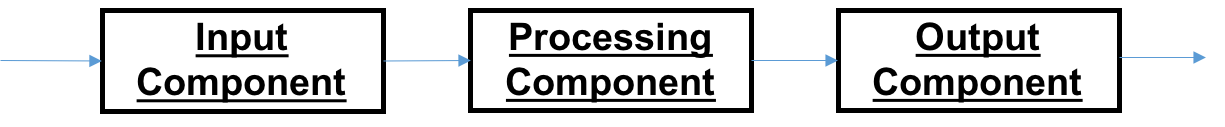
\includegraphics[width=0.8\textwidth]{includes/figures/fig_pipeline_simple}
  \caption{A simplistic overview of our pipeline design. Note the dataflow behaviour exhibited with each component output
  being an input of the following component.}
  \label{fig:pipeline_simple}
\end{figure}

We now have a simple design of the pipeline, however we are left with the questions of the output of the \textbf{Output Component},
the input of the \textbf{Input Component}, and the contents of each component.

The output of the \textbf{Output Component}
will simply be whatever extensions are needed to be made to the pipeline. Hence, rather than acting a sink, this component
will be an abstract interface which any extension needed will be able to adhere to to extend the pipeline. Designing the pipeline
in this manner directly addresses our third research question touched upon in Chapter 1, in~\sectref{sub:research_questions}.
This allows the output data to be dealt with in any manner required by the IRT team, whether it be stored for later
batch processing, or forwarded on for further realtime processing.

The input of the \textbf{Input Component} will be the data read from the sensors to which the pipeline is connected to.
The sensors generally would not be directly connected to the pipeline, so we could have another abstract interface here
that any sensor connects to, then the interface sends the data to the actual component. This allows data to be fed into
the pipeline from any type of sensor that is able to adhere to the interface.

The contents of each component is a larger task. For the \textbf{Processing Component}, it will want to be consisting
of a number of tasks, each of which are tasked to process the data in some manner before forwarding it onto whatever
the next specified task is. This, in itself, acts as a mini-pipeline where the core of processing will be done. Here
we will say that the \textbf{Processing Component} consists of $n$ sequential processing tasks. For the \textbf{Input Component},
the contents will consist of a task-like component tasked with passing data onto the processing tasks which make up the
\textbf{Processing Component}. The contents of the
\textbf{Output Component} will be as described previously: an abstract interface allowing for the extension of the pipeline.

This leaves us with a final pipeline design as illustrated in~\figref{fig:pipeline_whole}.

\begin{figure}[h]
  \centering
  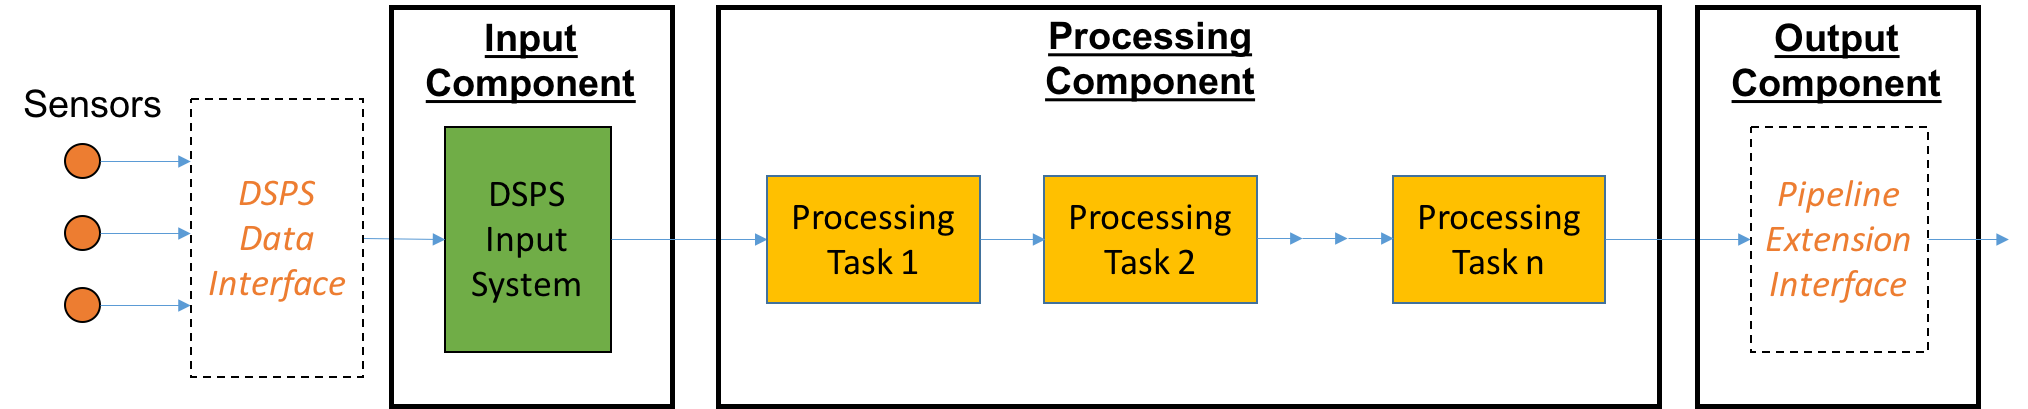
\includegraphics[width=0.8\textwidth]{includes/figures/fig_pipeline_whole}
  \caption{A complete overview of our pipeline design.}
  \label{fig:pipeline_whole}
\end{figure}

% subsection pipeline_design (end)


\subsection{Testing Environment Details} % (fold)
\label{sub:testing_environment_details}

\subsubsection{Details on Host System} % (fold)
\label{ssub:host_system}

The testing environment on which the prototype pipelines were implemented using each of the candidate DSPS technologies
is the same National eResearch Collaboration Tools and Resources (NeCTAR) cloud computing environment touched upon
briefly in Chapter 1. This cloud service platform is provided as an initiative by the Australian Government for researchers
that require the infrastructure\footnote{https://www.nectar.org.au/about-nectar}.

Our environment consists of a single NeCTAR cloud instance of which the details are specified in~\tabref{tab:control}.

\begin{table}[h]
\caption{Control system used for testing pipelines.}
\label{tab:control}
\centering
\begin{tabular}{ll}
\textbf{Distribution}         & Ubuntu GNU/Linux 14.04.2 LTS \\
\textbf{Kernel}               & Linux 3.13.0-36-generic    \\
\textbf{Architecture}         & x86\_64                    \\
\textbf{Virtual CPUs}         & 16                         \\
\textbf{Available RAM}        & 64 GB                      \\
\textbf{Available Disk Space} & 490 GB
\end{tabular}
\end{table}

The NeCTAR cloud instance utilises a single node upon which all processing is performed. In a real deployment, it is
common to use a full cluster upon which the pipeline would be deployed, where processing is shared between nodes. Due to
limited testing resources, all testing
has been performed on a single node cluster, however this remains a constant feature between all implementation and tests
performed in the project. Furthermore, the pipelines built upon
each of the candidate DSPS technologies are freely configurable to be deployed to run on arbitrarily sized clusters without
requiring changes to the underlying source code.

% subsubsection host_system (end)


\subsubsection{Details on Data Stream Processing System Technologies} % (fold)
\label{sub:setting_up_of_dsps_technologies}

While most details of each of the candidate DSPS technologies has previously been given in the last chapter, it is important
to outline the specific versions of each technology, as well as the programming languages used for implementation.

Version 0.9.0 of Samza was used for implementation of the prototype pipeline in Samza. At the time of implementation,
this was the major stable version of Samza, accepted as a top-level Apache project. Java, the only official programming
language supported by the Samza project, was used, using JDK 1.8.0 as the target implementation.

Version 0.9.4 of Storm was used for implementation of the prototype pipeline in Storm. As with Samza, this was also the
major stable version of Storm available. Java 8 was used as the implementation language, also compiling for the JDK 1.8.0.

Version 1.3.0 of Spark and the Spark Streaming extension were used for the Spark Streaming implementations. Prototype pipelines were
implemented in both Scala 2.9.2, targeting the JDK 1.8.0, and Python 2.7, which is made possible through the relatively new (as of Spark 1.2.0)
PySpark subsystem. Implementations for the Spark Streaming pipeline were built targeting both Spark JVM and PySpark due
to numerous undocumented claims that performance differs on both Spark implementations. These claims are addressed further
in the following chapter.

The specific JDK implementation for all tests was the Intel 64-bit OpenJDK 1.8.0 release 45 built and packaged for the GNU/Linux
distribution of Ubuntu 14.04.2 LTS.

% subsubsection setting_up_of_dsps_technologies (end)

% subsection testing_environment_details (end)


\subsection{Implementation of Pipelines in Data Stream Processing System Technologies} % (fold)
\label{sub:implementation_of_pipelines_in_dsps_technol}

\subsubsection{Samza} % (fold)
\label{ssub:impl_samza}

% subsubsection samza (end)


\subsubsection{Storm} % (fold)
\label{ssub:impl_storm}

% subsubsection storm (end)


\subsubsection{Spark Streaming (JVM Spark)} % (fold)
\label{ssub:impl_spark_streaming_jvm}

% subsubsection spark_streaming_ (end)


\subsubsection{Spark Streaming (PySpark)} % (fold)
\label{ssub:impl_spark_streaming_py}

% subsubsection spark_streaming_ (end)

% subsection implementation_of_pipelines_in_dsps_technol (end)


\subsection{Conclusion} % (fold)
\label{sub:implement_conclusion}

In conclusion this chapter has touched upon all details of implementation for each of the prototype pipelines.
We have detailed how each prototype data filtering pipeline has been built for each candidate system, ready
for subsequent tests and evaluation, of which will be discussed in the following chapter. Furthermore, the overall
design of the pipeline that has been implemented has been detailed along along with the details of the overall testing
environment upon which the pipelines are to be implemented.

% subsection conclusion (end)